\documentclass[t, aspectratio=169, 10pt]{beamer}
\usepackage{elmagTemplate}

% Utility packages
\newcommand\SLASH{\char`\\} % Used for command examples
\usepackage{array} % Array and tabular enhancements
\newcolumntype{C}[1]{>{\centering\arraybackslash}p{#1}} % Centered column type
\usepackage{amsmath, amssymb, amsfonts, physics, tabu, pgfplots}
\usepackage{tikz-3dplot}

\usepackage[school,simplified]{pgf-umlcd}
\usetikzlibrary{calc}
\usetikzlibrary{positioning}
\usetikzlibrary{shapes.geometric, arrows}
\usepackage{matlab-prettifier}
\usepackage{mathtools}

\tikzstyle{startstop} = [rectangle, rounded corners, 
minimum width=3cm, 
minimum height=1cm,
text centered, 
draw=black, 
fill=red!30]

\tikzstyle{io} = [trapezium, 
trapezium stretches=true, % A later addition
trapezium left angle=70, 
trapezium right angle=110, 
minimum width=3cm,
minimum height=1cm, text centered,
align = center,
draw=black, fill=blue!30]

\tikzstyle{process} = [rectangle, 
minimum width=3cm, 
minimum height=1cm, 
text centered, 
draw=black,
align=center,
fill=orange!30]


\tikzstyle{decision} = [diamond, 
minimum width=2cm, 
minimum height=1cm, 
text centered,
align=center,
draw=black, 
fill=green!30]
\tikzstyle{arrow} = [thick,->,>=stealth]

% Metadata
\title[\textsc{Matlab} competition task]{RFID login/registration demo}
\author[Tom\'a\v{s} Mach\'a\v{c}ek]{Tom\'a\v{s} Mach\'a\v{c}ek}
\date[\today]{\today}

\begin{document}

% Title Slide
\begin{frame}
    \titlepage
\end{frame}

% Outline
\begin{frame}{Outline}
    \tableofcontents
\end{frame}

\section{Project Description}
\begin{frame}{Introduction}
    \begin{itemize}
        \item A robust yet user-friendly registration and login system
        \item MQTT-based communication between the Raspberry Pi and Flask server
        \item A centralized database for banned users
    \end{itemize}
\end{frame}

\begin{frame}{Database structure}
    \begin{figure}[h!]
        \centering
        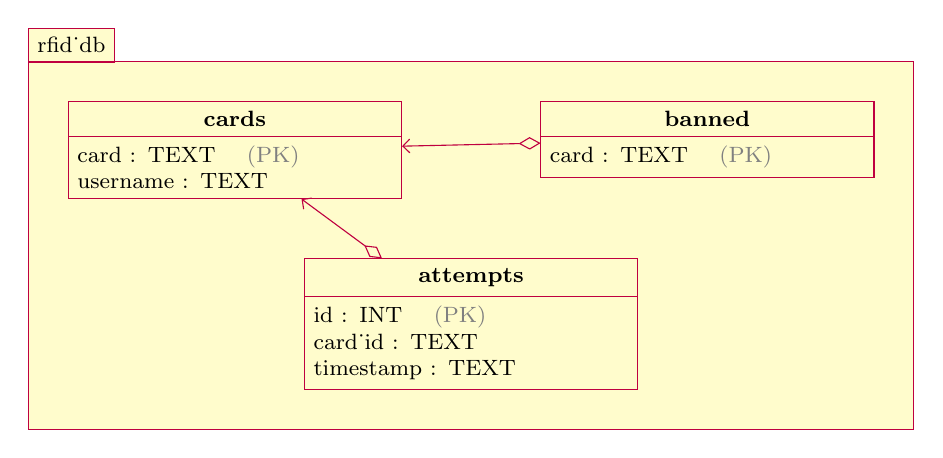
\begin{tikzpicture}[font=\footnotesize] % reduce fontsize
            \begin{package}{\detokenize{rfid_db}}

        % cards table
        \begin{class}[text width=4cm]{\detokenize{cards}}{0,0}
            \attribute{\detokenize{card} : TEXT \quad {\color{gray}(PK)}}
          \attribute{\detokenize{username} : TEXT}
        \end{class}

        % banned table, placed to the right
        \begin{class}[text width=4cm, xshift=6cm]{\detokenize{banned}}{0,0}
            \attribute{\detokenize{card} : TEXT \quad {\color{gray}(PK)}}
        \end{class}

        \begin{class}[text width=4cm, xshift=3cm, yshift=-2cm]{\detokenize{attempts}}{0,0}
            \attribute{\detokenize{id} : INT \quad {\color{gray}(PK)}}
            \attribute{\detokenize{card_id} : TEXT}
            \attribute{\detokenize{timestamp} : TEXT}
        \end{class}

            \aggregation{\detokenize{banned}}{}{}{\detokenize{cards}}
            \aggregation{\detokenize{attempts}}{}{}{\detokenize{cards}}

      \end{package}
        \end{tikzpicture}
    \end{figure}
\end{frame}


\section{Protocol Description}
\subsection{Registration}
\begin{frame}{Registration Workflow}
    \begin{itemize}
        \item The user enters a desired username.
        \item The Flask server publishes an MQTT message to initiate scanning on the Raspberry Pi.
        \item The user has up to three attempts to register. Registration will fail if:
            \begin{itemize}
                \item The card or username already exists.
                \item The card is listed in the banned-users database.
            \end{itemize}
    \end{itemize}
    \begin{figure}
        \centering
        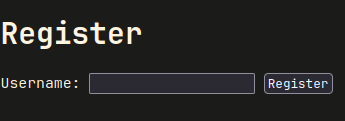
\includegraphics[height=3cm]{images/registration.png}
    \end{figure}
\end{frame}

\subsection{Login}
\begin{frame}{Login Workflow}
    \begin{itemize}
        \item The user presses the scan button to begin authentication.
        \item The system verifies that the card:
            \begin{enumerate}
                \item Is registered in the database.
                \item Is not present in the banned-users list.
            \end{enumerate}
    \end{itemize}
    \begin{figure}
        \centering
        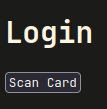
\includegraphics[height=3cm]{images/login.png}
    \end{figure}
\end{frame}

\subsection{Communication Protocol}
\begin{frame}{RFID Communication Protocol}
    \begin{itemize}
        \item The Flask server starts the sequence by publishing a “start” message via MQTT.
        \item The Raspberry Pi subscribes to the corresponding Mosquitto broker topic.
        \item A 3-second window opens for the RFID scan.
        \item Upon a successful scan, the Raspberry Pi publishes the RFID tag data with QoS=1.
    \end{itemize}
\end{frame}

\section*{Questions}
\begin{frame}
    \centering
    \vspace{2cm}
    {\Huge Questions?}
\end{frame}

\end{document}

